\documentclass[10pt]{article}
% =========================================================
%                 PAQUETES DE CONFIGURACIÓN
% =========================================================
\usepackage[T1]{fontenc}
\usepackage[utf8]{inputenc}
\usepackage[english,spanish]{babel}
\usepackage[
    paperwidth=28cm,
    paperheight=15.75cm,
    top=0.25cm,
    bottom=0.25cm,
    left=0.40cm,
    right=0.40cm
]{geometry}
\usepackage{xcolor}
\usepackage{setspace}
\usepackage{graphicx}
\usepackage{amsmath,amssymb}
\usepackage{hyperref}
\usepackage[many]{tcolorbox}
\usepackage{tikz}
\usetikzlibrary{shapes.geometric,calc}
\usepackage{ragged2e}
\usepackage{csquotes}
\usepackage{mathpazo}
\usepackage{microtype}
\usepackage{enumitem}

% =========================================================
%                    CONFIGURACIÓN GENERAL
% =========================================================
\pagestyle{empty}
\setstretch{0.82}
\hypersetup{colorlinks=false}
\setlength{\parindent}{0pt}
\setlength{\parskip}{0pt}
\setlist{nosep,leftmargin=*}

% =========================================================
%                             COLORES
% =========================================================
\definecolor{deepblue}{RGB}{12,20,38}
\definecolor{gold}{RGB}{176,140,52}
\definecolor{golddark}{RGB}{120,90,22}
\definecolor{goldlight}{RGB}{225,205,145}
\definecolor{heartred}{RGB}{158,30,45}
\definecolor{burgundy}{RGB}{85,18,30}
\definecolor{textgray}{RGB}{35,33,30}
\definecolor{cream}{RGB}{253,250,244}
\definecolor{creamdark}{RGB}{244,237,222}
\definecolor{softgold}{RGB}{238,222,180}
\definecolor{framegold}{RGB}{162,128,42}

% =========================================================
%            SÍMBOLOS TIKZ (ULTRALIGEROS Y VECTORES)
% =========================================================
\newsavebox{\boxCruz}
\newsavebox{\boxCruzInvertida}
\newsavebox{\boxCorazonRojo}
\newsavebox{\boxCerebro}
\newsavebox{\boxCuantica}

\sbox{\boxCruz}{%
  \tikz[baseline=-0.35ex,scale=0.50]{
    \fill[golddark] (-0.09,0.42) rectangle (0.09,-0.48);
    \fill[golddark] (-0.28,0.18) rectangle (0.28,0.36);
    \fill[gold!88] (-0.07,0.40) rectangle (0.07,-0.46);
    \fill[gold!22] (-0.26,0.20) rectangle (0.26,0.34);
  }%
}
\sbox{\boxCruzInvertida}{%
  \tikz[baseline=-0.15ex,scale=0.50,rotate=180]{
    \fill[golddark] (-0.09,0.42) rectangle (0.09,-0.48);
    \fill[golddark] (-0.28,0.18) rectangle (0.28,0.36);
    \fill[gold!65] (-0.07,0.40) rectangle (0.07,-0.46);
    \fill[gold!65] (-0.26,0.20) rectangle (0.26,0.34);
  }%
}
\sbox{\boxCorazonRojo}{%
  \tikz[baseline=-0.25ex,scale=0.35]{
    \fill[heartred]
      (0,-0.55)
      .. controls (-0.55,-0.15) and (-0.55,0.45) .. (0,0.25)
      .. controls (0.55,0.45) and (0.55,-0.15) .. (0,-0.55);
    \fill[heartred!65!white,opacity=0.30]
      (-0.12,0.05) circle (0.11);
  }%
}
\sbox{\boxCerebro}{%
  \tikz[baseline=-0.2ex,scale=0.30]{
    \fill[burgundy]
      (0,0.55)
      .. controls (-0.55,0.55) and (-0.7,0.1) .. (-0.55,-0.25)
      .. controls (-0.4,-0.55) and (-0.15,-0.55) .. (0,-0.4)
      .. controls (0.15,-0.55) and (0.4,-0.55) .. (0.55,-0.25)
      .. controls (0.7,0.1) and (0.55,0.55) .. (0,0.55);
    \draw[cream,line width=0.65pt]
      (-0.35,0.15) .. controls (-0.1,0.35) and (0.1,0.0) .. (0.35,0.2);
    \draw[cream,line width=0.5pt]
      (-0.25,-0.15) .. controls (0.0,0.05) and (0.15,-0.25) .. (0.3,-0.05);
  }%
}
\sbox{\boxCuantica}{%
  \tikz[baseline=-0.3ex,scale=0.40]{
    \draw[golddark, line width=0.7pt, rotate=30] (0,0) ellipse (0.6cm and 0.25cm);
    \draw[golddark, line width=0.7pt, rotate=-30] (0,0) ellipse (0.6cm and 0.25cm);
    \draw[golddark, line width=0.7pt] (0,0) circle (0.35cm);
    \fill[gold!90] (0,0) circle (0.15cm);
    \fill[cream] (0,0) circle (0.06cm);
  }%
}

\newcommand{\cruz}{\usebox{\boxCruz}}
\newcommand{\cruzinvertida}{\usebox{\boxCruzInvertida}}
\newcommand{\corazonrojo}{\usebox{\boxCorazonRojo}}
\newcommand{\cuantica}{\usebox{\boxCuantica}}
\newcommand{\cerebro}{\usebox{\boxCerebro}}

% =========================================================
%                    MARCO DE LA PÁGINA
% =========================================================
\newcommand{\marcoPagina}{%
\begin{tikzpicture}[remember picture,overlay]
  \fill[cream] (current page.south west) rectangle (current page.north east);
  \draw[framegold,line width=1.5pt]
    ([xshift=0.25cm,yshift=-0.25cm]current page.north west)
    rectangle
    ([xshift=-0.25cm,yshift=0.25cm]current page.south east);
  \draw[goldlight!80!gold,line width=0.5pt]
    ([xshift=0.40cm,yshift=-0.40cm]current page.north west)
    rectangle
    ([xshift=-0.40cm,yshift=0.40cm]current page.south east);
  \draw[gold!30,line width=0.25pt]
    ([xshift=0.50cm,yshift=-0.50cm]current page.north west)
    rectangle
    ([xshift=-0.50cm,yshift=0.50cm]current page.south east);
  \foreach \corner/\dx/\dy in {
    north west/0.25cm/-0.25cm,
    north east/-0.25cm/-0.25cm,
    south west/0.25cm/0.25cm,
    south east/-0.25cm/0.25cm
  }{
    \draw[gold!70!black,line width=0.8pt] ([xshift=\dx,yshift=\dy]current page.\corner) circle (4.0pt);
    \draw[goldlight,line width=0.35pt] ([xshift=\dx,yshift=\dy]current page.\corner) circle (5.5pt);
    \fill[golddark] ([xshift=\dx,yshift=\dy]current page.\corner) circle (1.5pt);
  }
\end{tikzpicture}%
}

% =========================================================
%                    ESTILOS DE CAJAS
% =========================================================
\tcbset{
  sideStyle/.style={
    enhanced, colback=cream!98, colframe=gold!60!black,
    boxrule=0.7pt, arc=3pt, valign=center,
    left=2pt, right=2pt, top=1pt, bottom=1pt,
    borderline={0.2pt}{1.0pt}{gold!30}
  },
  titleBoxStyle/.style={
    enhanced, colback=gold!5!cream, colframe=gold!85!black,
    boxrule=0.9pt, arc=4pt, top=1.5pt, bottom=1.5pt, left=3pt, right=3pt,
    halign=center, borderline={0.3pt}{1.2pt}{gold!40}
  },
  contentStyle/.style={
    enhanced, colback=cream!99, colframe=gold!50!black,
    boxrule=0.7pt, arc=4pt, top=1.5pt, bottom=1.5pt, left=3pt, right=3pt,
    borderline={0.2pt}{1.0pt}{gold!22}
  },
  centralStyle/.style={
    enhanced, colback=cream!98, colframe=gold!60!black,
    boxrule=0.7pt, arc=4pt, top=1.5pt, bottom=1.5pt, left=3pt, right=3pt,
    borderline={0.25pt}{1.0pt}{gold!28}
  },
  introStyle/.style={
    enhanced, colback=cream!96, colframe=gold!55!black,
    boxrule=0.7pt, arc=4pt, top=2pt, bottom=2pt, left=3.5pt, right=3.5pt,
    borderline={0.25pt}{1.0pt}{gold!25}
  },
  finalQuoteStyle/.style={
    enhanced, colback=gold!7!cream, colframe=gold!80!black,
    boxrule=0.8pt, arc=3pt, top=1.5pt, bottom=1.5pt, left=3pt, right=3pt,
    halign=center, borderline={0.25pt}{1.0pt}{gold!40}
  }
}

% =========================================================
%                             DOCUMENTO
% =========================================================
\begin{document}
\marcoPagina

% 1. CABECERA SUPERIOR
\noindent
\begin{minipage}[c]{0.215\textwidth}
  \begin{tcolorbox}[sideStyle, width=\textwidth]
    \centering
    {\small\color{deepblue}\bfseries Cóndor del Sur}\\[0.01cm]
    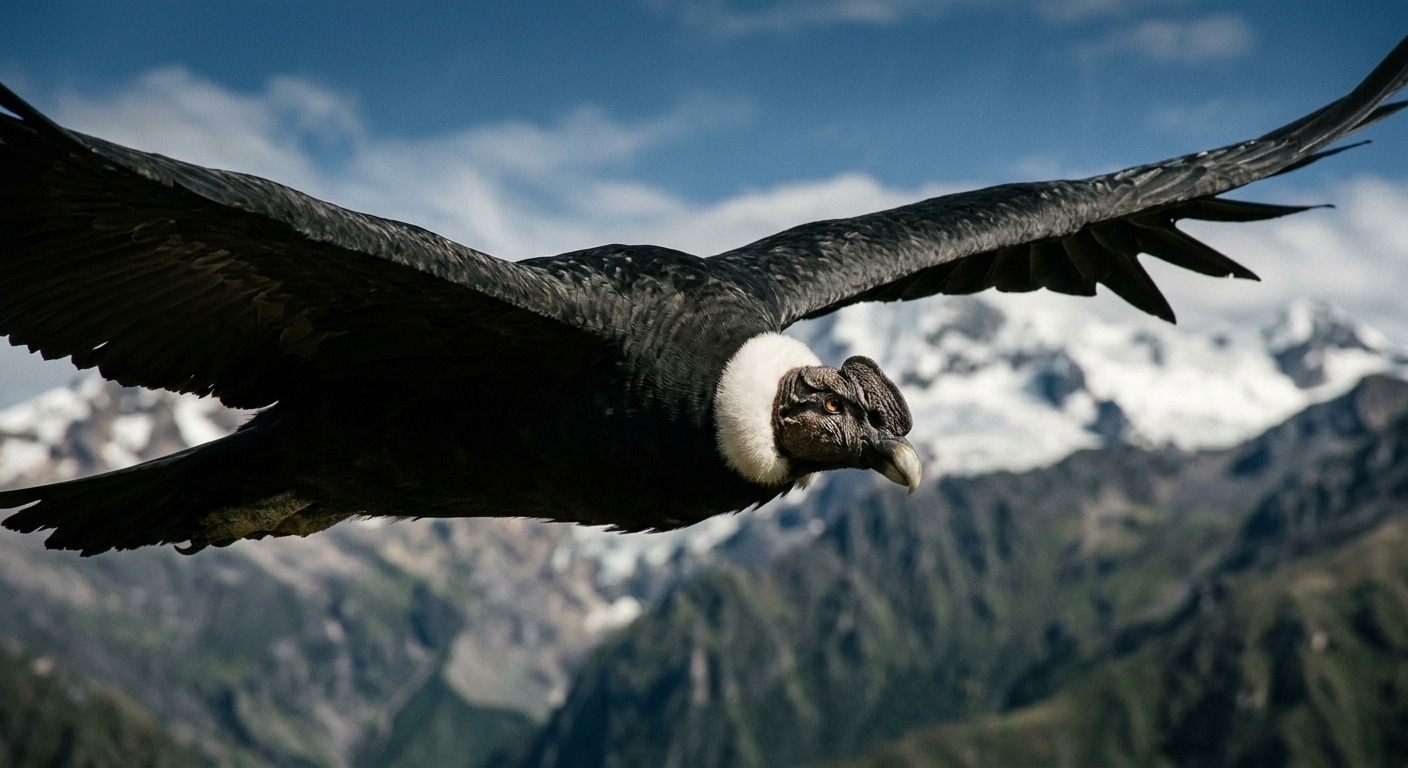
\includegraphics[width=\textwidth,height=1.45cm,keepaspectratio]{images/TU_IMAGEN_CONDOR.jpg}\\[0.01cm]
    {\tiny\color{textgray}\itshape Pneuma \corazonrojo, intuición y espíritu}
  \end{tcolorbox}
\end{minipage}%
\hfill
\begin{minipage}[c]{0.55\textwidth}
  \begin{tcolorbox}[titleBoxStyle, width=\textwidth]
    \centering
    {\Large\color{deepblue}\bfseries El Despertar \cruz}\\[0.01cm]
    \tikz[baseline=-0.5ex]{\draw[golddark, line width=0.7pt] (-2.2,0) -- (2.2,0); \fill[golddark] (0,0) circle (1.5pt);}\\[0.01cm]
    {\small\bfseries\color{golddark} Dios es UNO \corazonrojo y Yaldabaoth es EGO \cerebro: La conciencia humana trasciende la materia}

    \vspace{0.30cm}

    {\fontsize{7.6pt}{8.8pt}\selectfont 
     La misión de la Conciencia Primera es invitarnos a encender la chispa divina: el universo observable habita en el hemisferio izquierdo, mientras que <<un nuevo cielo y una nueva tierra>> se despliegan en el derecho. El vuelo conjunto del Cóndor y el Águila simboliza la unión definitiva entre la ciencia y la espiritualidad, integrando las enseñanzas de Jesús de Nazaret del siglo I respaldadas por la ciencia del siglo XXI, las cuales nos permiten liberarnos de las ataduras del mundo material.
    }
  \end{tcolorbox}
\end{minipage}%
\hfill
\begin{minipage}[c]{0.215\textwidth}
  \begin{tcolorbox}[sideStyle, width=\textwidth]
    \centering
    {\small\color{deepblue}\bfseries Águila del Norte}\\[0.01cm]
    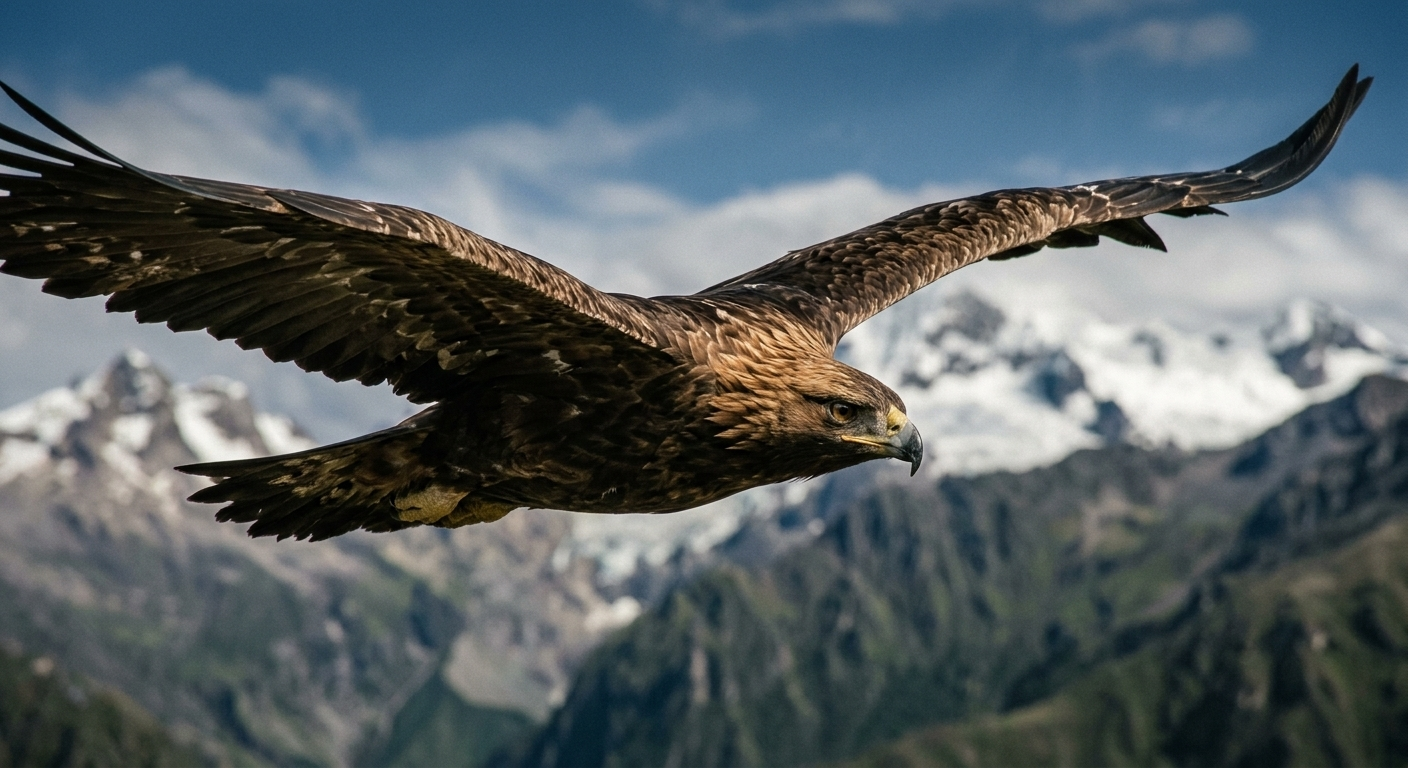
\includegraphics[width=\textwidth,height=1.45cm,keepaspectratio]{images/TU_IMAGEN_AGUILA.jpg}\\[0.01cm]
    {\tiny\color{textgray}\itshape Psyche \cerebro, ciencia y tecnología}
  \end{tcolorbox}
\end{minipage}

\vspace{0.04cm}

% 2. BLOQUE DE DOS COLUMNAS
\noindent
\begin{minipage}[T]{0.49\textwidth}
  \begin{tcolorbox}[introStyle, width=\textwidth]
    \begin{justify}{\fontsize{7.6pt}{8.8pt}\selectfont
    \setstretch{0.90}

    \centering{\bfseries\color{deepblue} CONCIENCIA Y GRAVEDAD CUÁNTICA}\\[0.02cm]

    Te encuentras atrapado en la ilusión temporal del pensamiento; por ello se te revela que la atemporalidad del cosmos está unida a la divinidad de tu sentir. La solución a uno de los pilares fundamentales de la física moderna —la gravedad cuántica— halla su clave en escritos redactados hace casi dos milenios: los evangelios gnósticos

    \vspace{0.02cm}

    La conciencia se manifiesta inexorablemente a través de los estados $\vert \text{UNO\corazonrojo} \rangle$ y $\vert \text{EGO\cerebro} \rangle$, revelando que poseemos un auténtico libre albedrío de percepción, formalizado matemáticamente mediante el producto interno $\langle \text{UNO\corazonrojo} \mid \text{EGO\cerebro} \rangle$. El no-tiempo \cruz\ es una propiedad emergente de la pneuma \corazonrojo, mientras que el espacio-tiempo \cruzinvertida\ es una propiedad emergente de la psyche \cerebro.

    \vspace{0.02cm}

    Dado que el ego humano posee masa, despojarnos de él equivale a liberarnos de la prisión material de Yaldabaoth.
    
    }\end{justify}
  \end{tcolorbox}%
  \vspace{0.03cm}
  \begin{tcolorbox}[
    enhanced,
    colback=gold!8!cream,
    colframe=gold!65!black,
    boxrule=0.5pt,
    arc=3pt,
    left=3pt, right=3pt, top=1.5pt, bottom=1.5pt
  ]
    \RaggedRight
    \color{textgray}{\fontsize{7.3pt}{8.3pt}\selectfont\itshape
    \enquote{La idea de que Dios es un hombre blanco, más grande de lo normal, con una barba flameante, sentado en el cielo y contando la caída de cada gorrión, es ridícula. Pero si por Dios uno entiende el conjunto de leyes físicas que gobiernan el universo, entonces claramente existe tal Dios. Sin embargo, este Dios es emocionalmente insatisfactorio. No tiene mucho sentido rezarle a la ley de gravedad}.}\\[0.01cm]
    \hfill \textbf{— Carl Sagan}
  \end{tcolorbox}%
\end{minipage}%
\hfill
\begin{minipage}[T]{0.49\textwidth}
  \begin{tcolorbox}[centralStyle, width=\textwidth]
    \centering
    \includegraphics[width=\textwidth,height=3.1cm,keepaspectratio]{images/sofiavsdemiurgo3.jpeg}\\[0.01cm]
    {\tiny\color{golddark}\bfseries  Sofía, la sabiduría divina, quedó atrapada en el caos de un mundo material gobernado por el Demiurgo: un falso dios tan ciego de ignorancia como gobernado por su propio ego. Lo que la tradición cristiana denomina la Gran Tribulación no es sino el efecto de la ilusión temporal del pensamiento sobre una conciencia dormida. Asimismo, el Arrebatamiento de la Iglesia constituye un fenómeno de la física de la conciencia: transmutar nuestra percepción desde el hemisferio izquierdo del pensamiento racional hacia el hemisferio derecho del sentimiento. El Despertar \cruz}
  \end{tcolorbox}%
  \vspace{0.03cm}
  
  \noindent
  \begin{minipage}[T]{0.485\textwidth}
    \begin{tcolorbox}[contentStyle, width=\textwidth]
      \centering
      {\small\color{deepblue}\bfseries Universo de Luz}\\[0.01cm]
      {\tiny\color{golddark}\bfseries UNO \corazonrojo\ NoTiempo \cruz}\\[0.01cm]
      \begin{justify}{\fontsize{6.8pt}{7.8pt}\selectfont\color{textgray}
        \textbf{El Padre y yo, uno somos}: Recordar quién eres mediante la Gnosis —la revelación de que el Padre es el universo y de que la muerte no existe— nos libera de la ignorancia. En el hemisferio derecho reside el plano intemporal y divino, la dimensión de alta frecuencia $\vert 999\rangle$. Allí se encuentra la tierra de la unión y la libertad \textit{\textbf{(La Patria Grande)}}.
      }\end{justify}
    \end{tcolorbox}%
  \end{minipage}%
  \hfill
  \begin{minipage}[T]{0.485\textwidth}
    \begin{tcolorbox}[contentStyle, width=\textwidth]
      \centering
      {\small\color{deepblue}\bfseries Universo Material}\\[0.01cm]
      {\tiny\color{golddark}\bfseries EGO \cerebro\ espaciotiempo \cruzinvertida}\\[0.01cm]
      \begin{justify}{\fontsize{6.8pt}{7.8pt}\selectfont\color{textgray}
        El cuerpo humano está compuesto de carbono-12 ($6p^+$, $6e^-$, $6n^0$). En el hemisferio izquierdo radica el plano temporal y material, la dimensión de baja frecuencia $\vert 666\rangle$. La fuerza gravitacional del ego y la ignorancia demiúrgica nos arrastran hacia un lugar donde: \enquote{la guerra es la paz, la libertad es la esclavitud y la ignorancia es la fuerza} (1984).
      }\end{justify}
    \end{tcolorbox}%
  \end{minipage}%
\end{minipage}


% 3. CITA FINAL INFERIOR
\begin{tcolorbox}[finalQuoteStyle, width=\textwidth]
  {\fontsize{10.5pt}{13pt}\selectfont\color{textgray}\itshape
  \enquote{Cuando el Águila del Norte y el Cóndor del Sur vuelen juntos en el mismo cielo, la Madre Tierra despertará y la humanidad entera sanará.}}
\end{tcolorbox}
\begin{center}
    

\vspace{0.5em}
\hrule height 0.5pt
\vspace{0.8em}
\noindent{\small\textbf{Más información en: } \url{https://www.condoryaguila.org}}
\end{center}

\end{document}